\section{Final Tables for Four Lepton Analyses}
The summarized results are presented in three tables: 
\begin{itemize}
\item Table~\ref{tab:fourLeptonResults} contains observed yields  and background prediction 
for each search region in the four lepton channels
\end{itemize}

The graphical representation of the results is shown in 
Figures~\ref{fig:L4OSSF0tau0},~\ref{fig:L4OSSF0tau1},~\ref{fig:L4OSSF1offZtau0},~\ref{fig:L4OSSF1onZtau0},
~\ref{fig:L4OSSF1offZtau1},~\ref{fig:L4OSSF1onZtau1},~\ref{fig:L4OSSF2offZtau0}, and~\ref{fig:L4OSSF2onZtau0}.

%==========================================================================================
\begin{figure}[htp]
\begin{center}
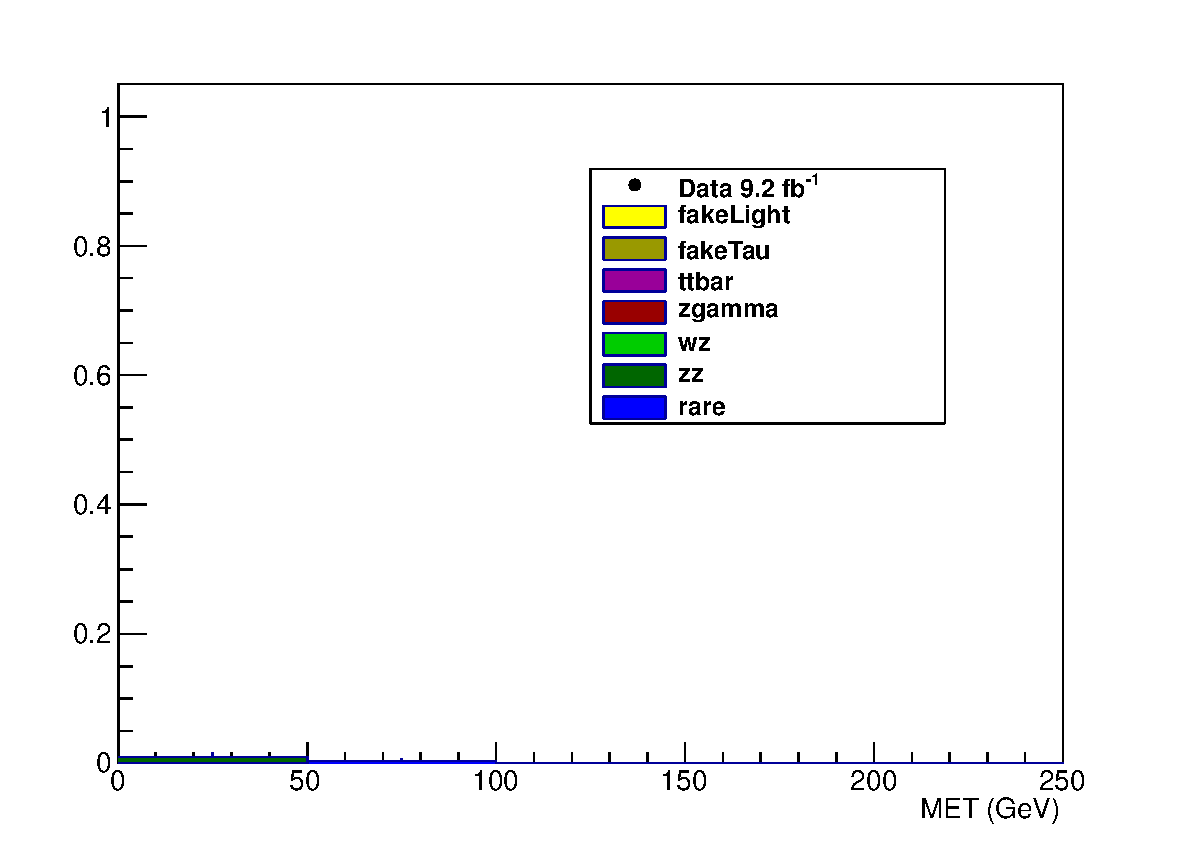
\includegraphics[width=0.63\textwidth]{plots/4L_MET_dist_offZ_ossf0_tau0_note.pdf}
\caption{Observed yields and predicted backgrounds for four lepton events with no OSSF pairs and zero taus.}
\label{fig:L4OSSF0tau0}
\end{center}
\end{figure}
%==========================================================================================
%==========================================================================================
\begin{figure}[htp]
\begin{center}
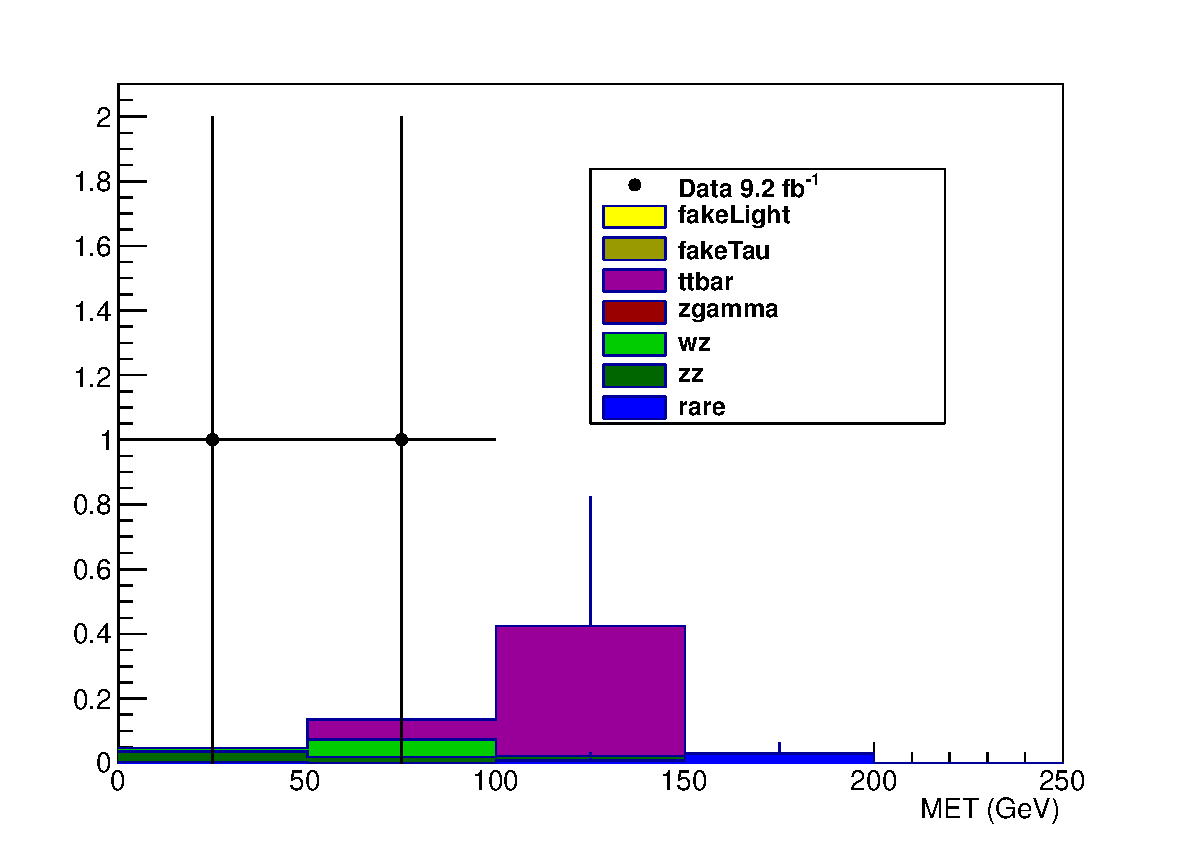
\includegraphics[width=0.63\textwidth]{plots/4L_MET_dist_offZ_ossf0_tau1_note.pdf}
\caption{Observed yields and predicted backgrounds for four lepton events with no OSSF pairs and one tau.}
\label{fig:L4OSSF0tau1}
\end{center}
\end{figure}
%==========================================================================================
%==========================================================================================
\begin{figure}[htp]
\begin{center}
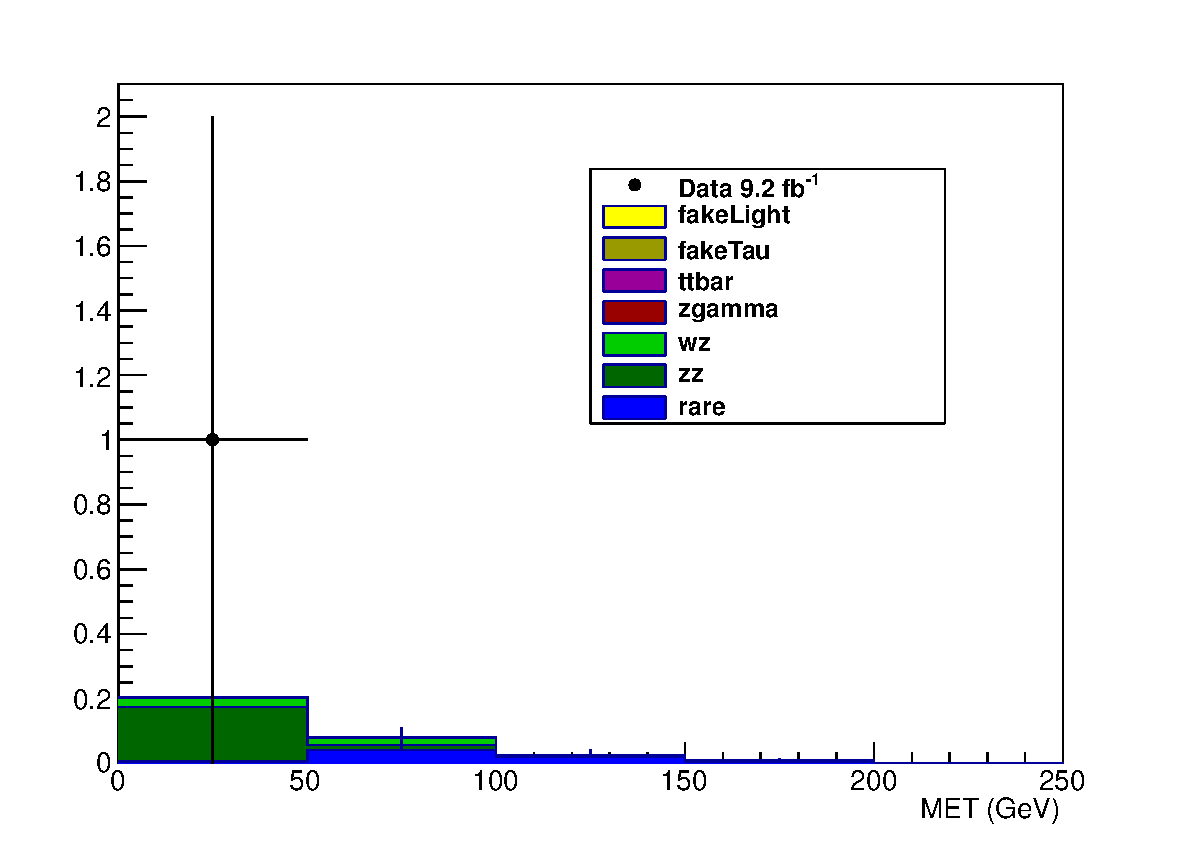
\includegraphics[width=0.8\textwidth]{plots/4L_MET_dist_offZ_ossf1_tau0_note.pdf}
\caption{Observed yields and predicted backgrounds for four lepton events with one OSSF pair offZ and zero taus.}
\label{fig:L4OSSF1offZtau0}
\end{center}
\end{figure}
%==========================================================================================
%==========================================================================================
\begin{figure}[htp]
\begin{center}
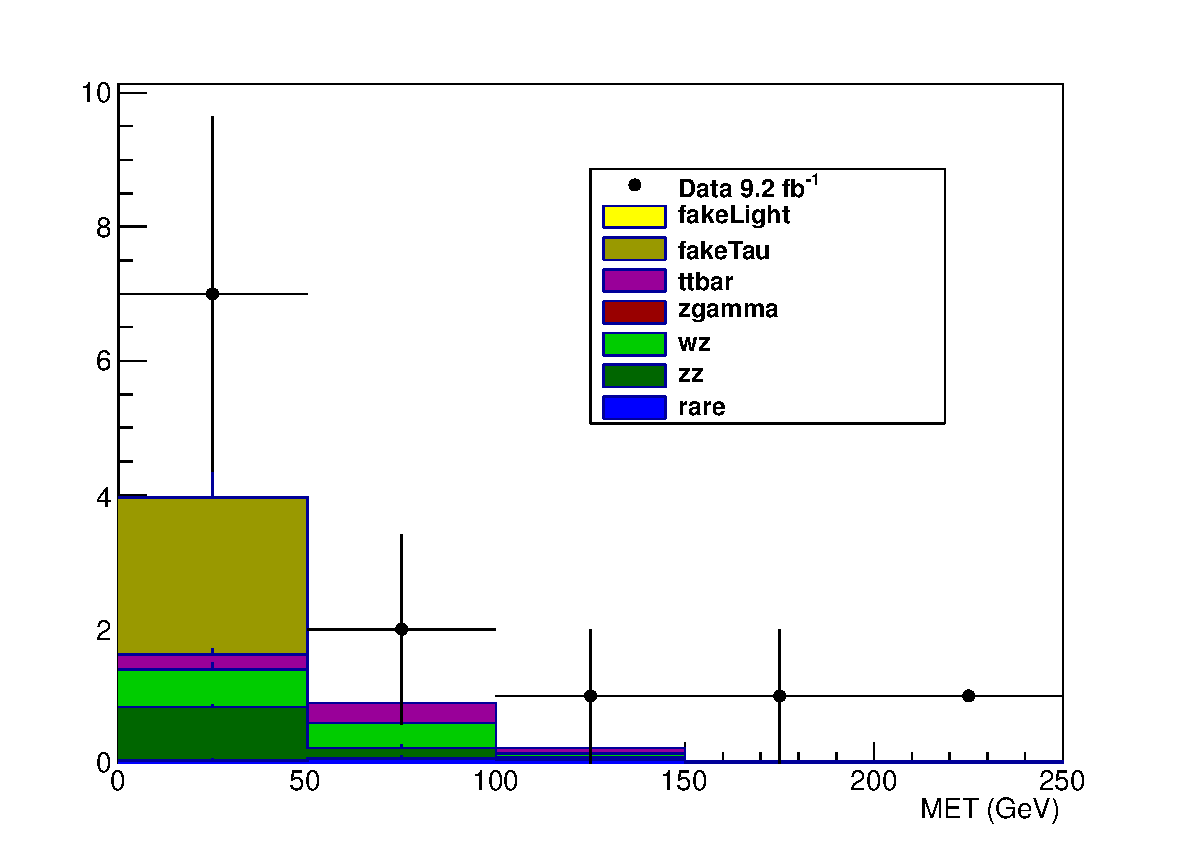
\includegraphics[width=0.8\textwidth]{plots/4L_MET_dist_offZ_ossf1_tau1_note.pdf}
\caption{Observed yields and predicted backgrounds for four lepton events with one OSSF pair off Z and one tau.}
\label{fig:L4OSSF1offZtau1}
\end{center}
\end{figure}
%==========================================================================================
%==========================================================================================
\begin{figure}[htp]
\begin{center}
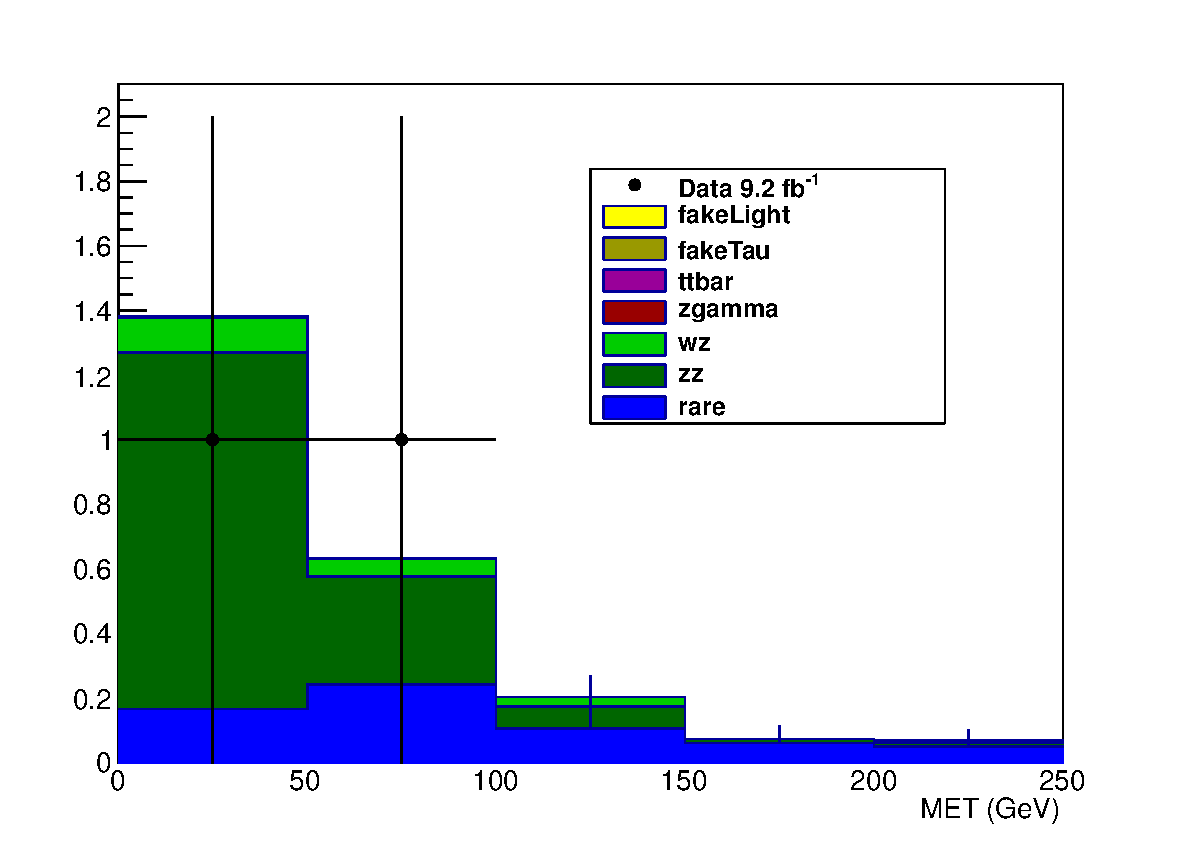
\includegraphics[width=0.8\textwidth]{plots/4L_MET_dist_onZ_ossf1_tau0_note.pdf}
\caption{Observed yields and predicted backgrounds for four lepton events with one OSSF pair on Z and zero taus.}
\label{fig:L4OSSF1onZtau0}
\end{center}
\end{figure}
%==========================================================================================
%==========================================================================================
\begin{figure}[htp]
\begin{center}
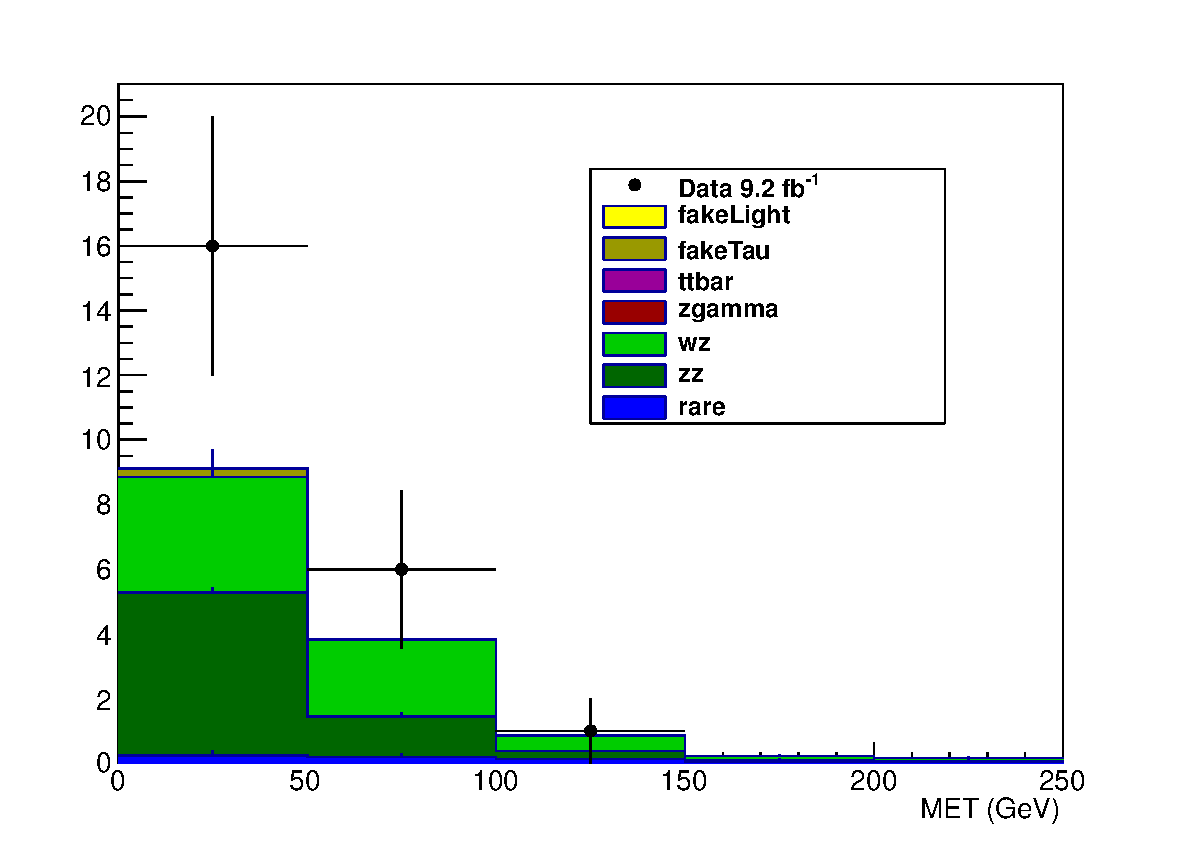
\includegraphics[width=0.8\textwidth]{plots/4L_MET_dist_onZ_ossf1_tau1_note.pdf}
\caption{Observed yields and predicted backgrounds for four lepton events with one OSSF pair on Z and one tau.}
\label{fig:L4OSSF1onZtau1}
\end{center}
\end{figure}
%==========================================================================================
%==========================================================================================
\begin{figure}[htp]
\begin{center}
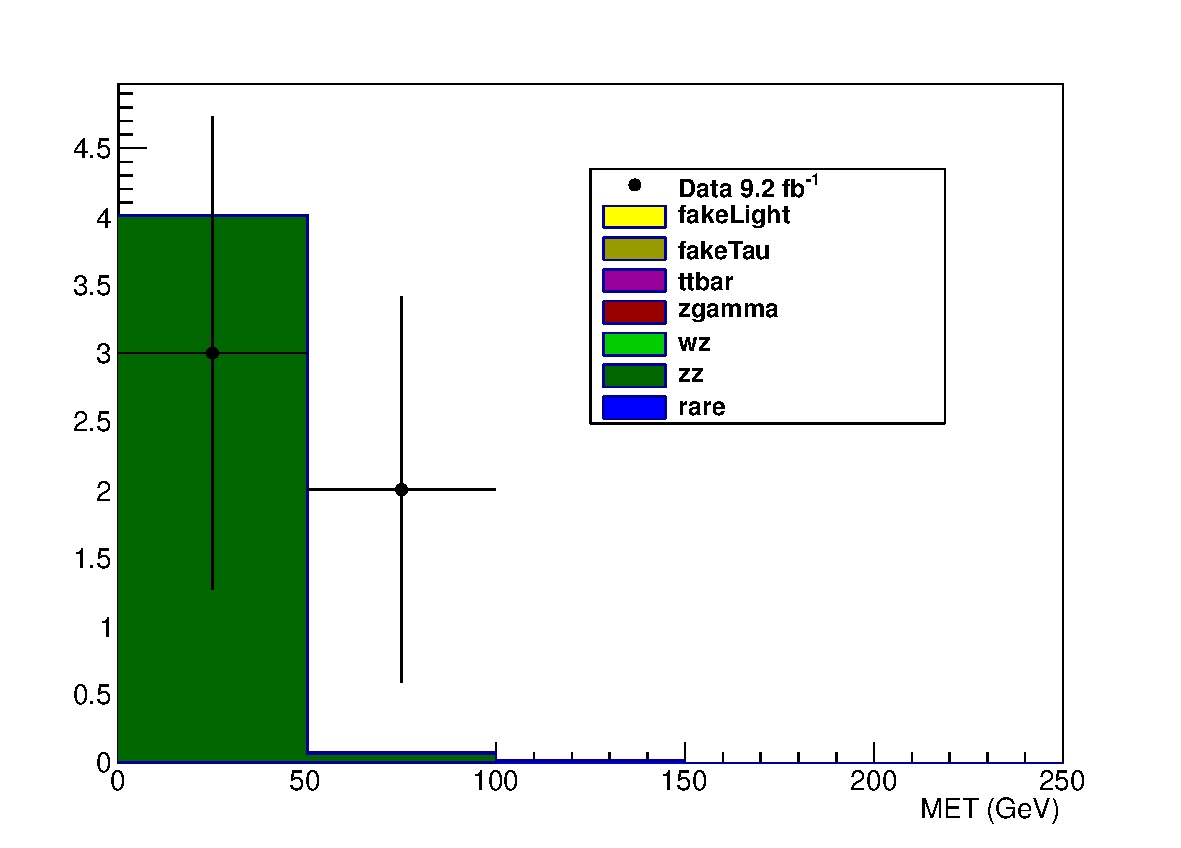
\includegraphics[width=0.8\textwidth]{plots/4L_MET_dist_offZ_ossf2_tau0_note.pdf}
\caption{Observed yields and predicted backgrounds for four lepton events with two OSSF pairs offZ and zero taus.}
\label{fig:L4OSSF2offZtau0}
\end{center}
\end{figure}
%==========================================================================================
%==========================================================================================
\begin{figure}[htp]
\begin{center}
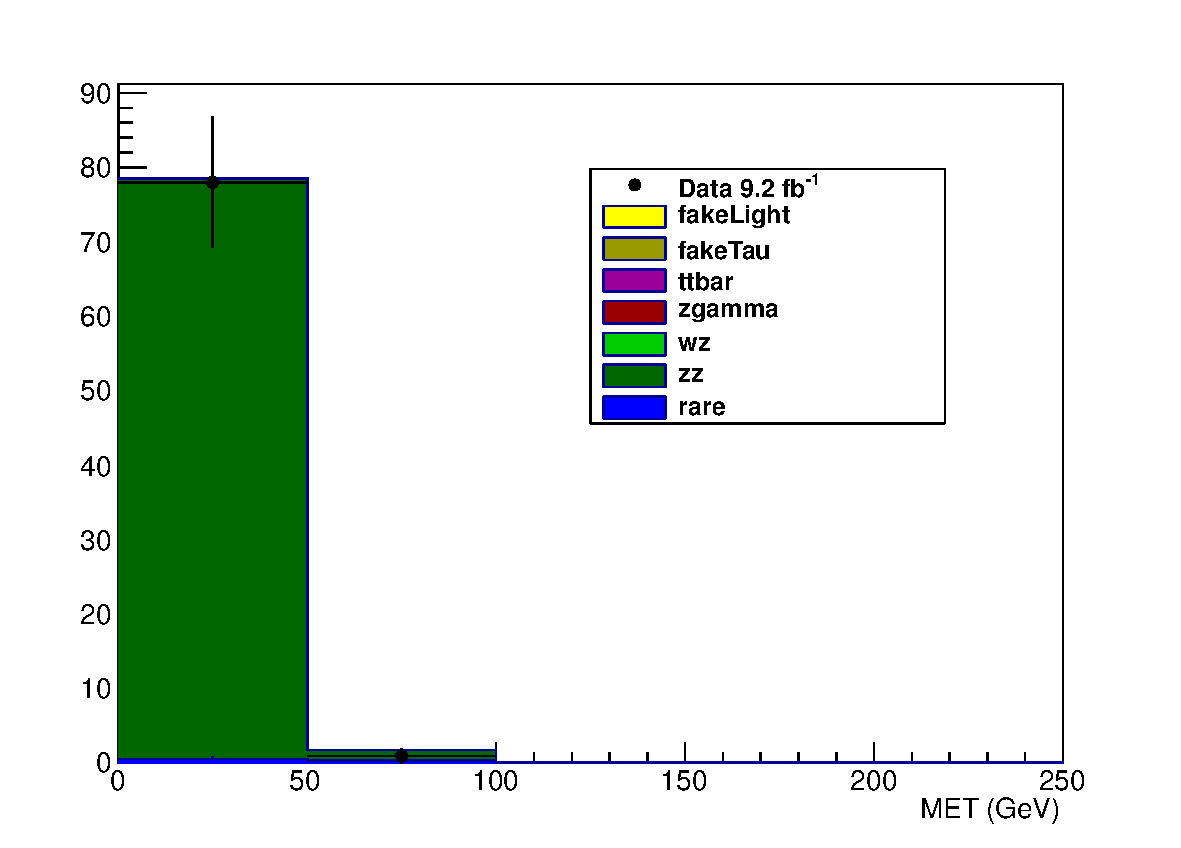
\includegraphics[width=0.8\textwidth]{plots/4L_MET_dist_onZ_ossf2_tau0_note.pdf}
\caption{Observed yields and predicted backgrounds for four lepton events with two OSSF pairs onZ and zero taus.}
\label{fig:L4OSSF2onZtau0}
\end{center}
\end{figure}
%==========================================================================================
%==========================================================================================
\begin{figure}[h!]
\begin{center}
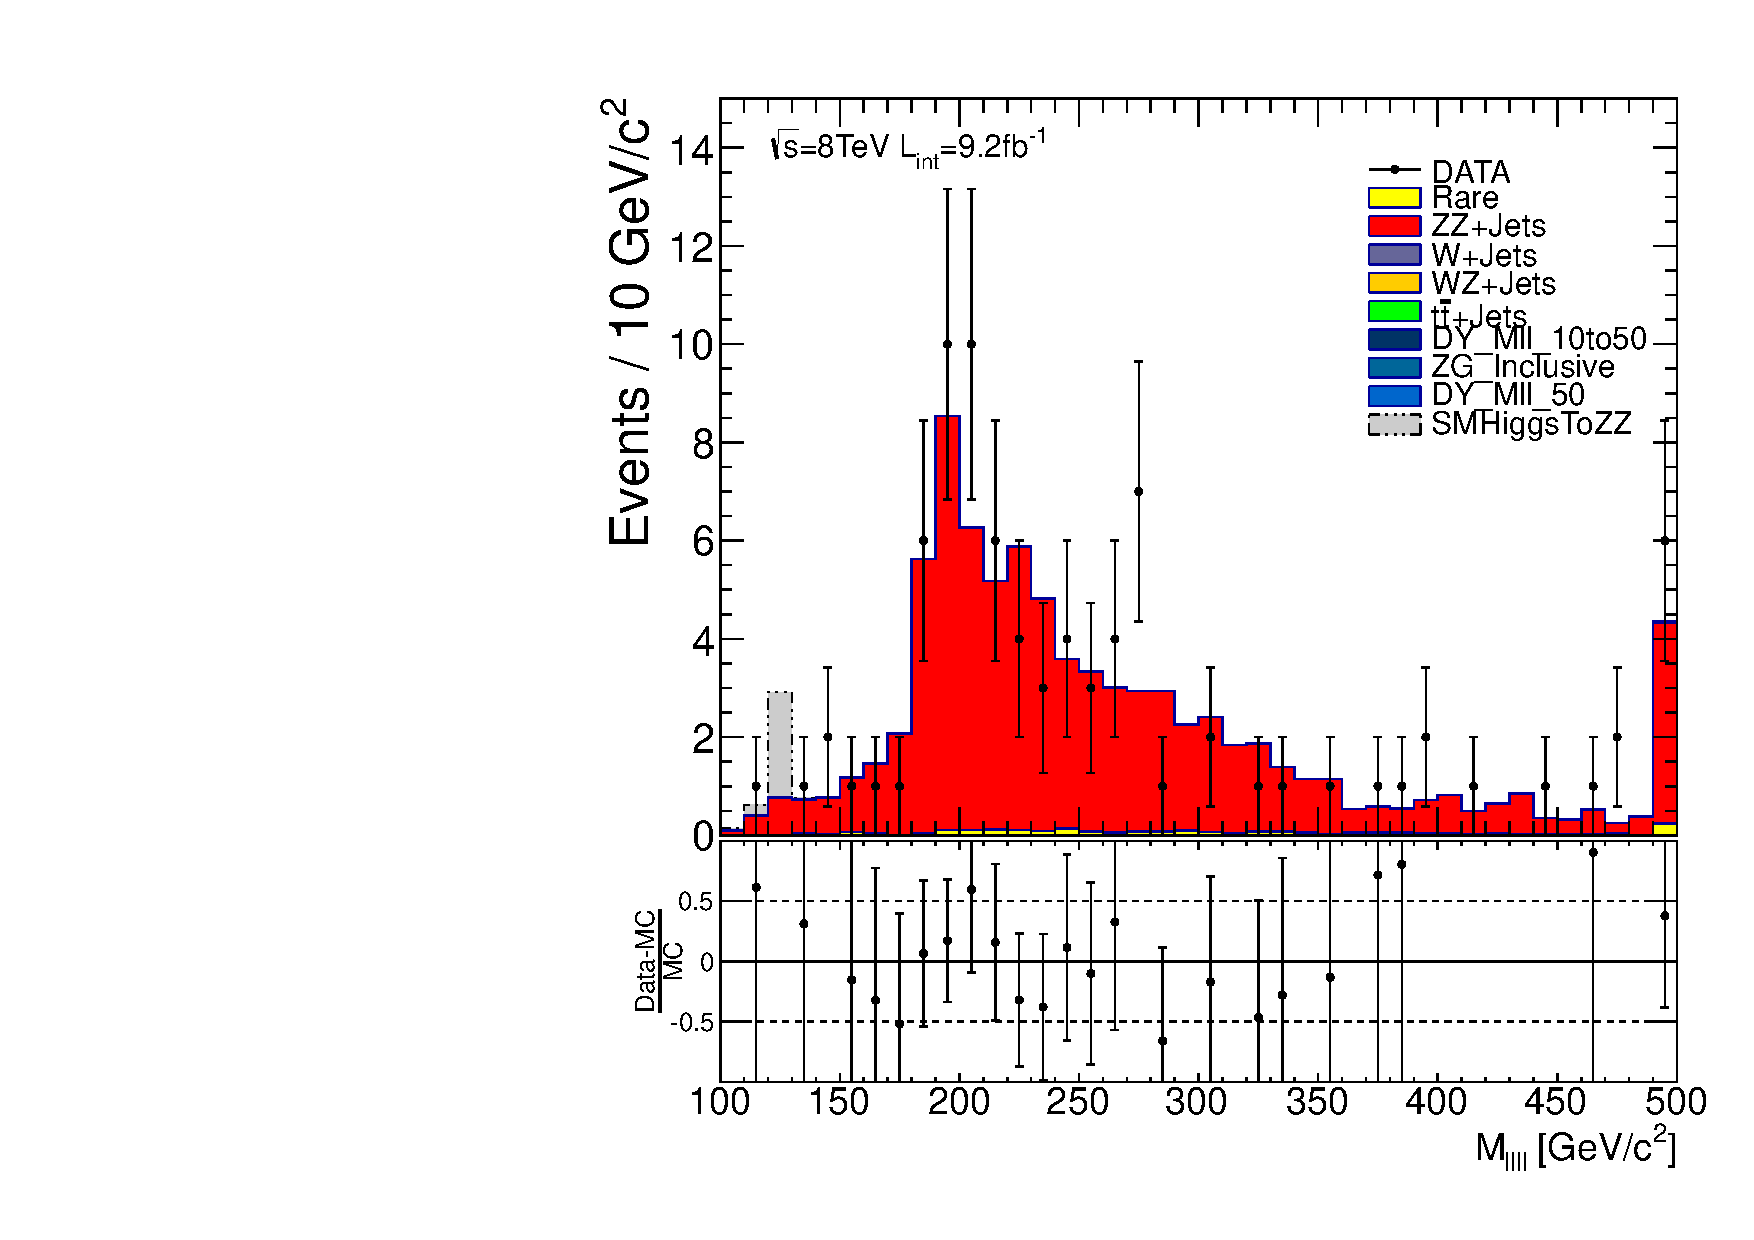
\includegraphics[width=0.8\textwidth]{plots/h_Four_invm4l_2OSSF.pdf}
\caption{Invariant mass of all four leptons in the events with four leptons, two OSSF pairs, and zero leptons. 
For comparison, we show the Higgs to ZZ to 4L expected signal.}
\label{fig:L4OSSF2Mass4L}
\end{center}
\end{figure}
%==========================================================================================

\newpage
\begin{table}[htp]
\begin{center}
\caption{\label{tab:fourLeptonResults} Four lepton backgrounds and observed yields. Backgrounds are given with statistical and systematic uncertainties, in that order.}
%\scriptsize
%\footnotesize
\tiny
\begin{tabular}{|c|c|c|ccccc|}\hline\hline
$\ETmiss$ (GeV) & Observed & Total Bkg &  $Z\gamma^{*}$ &  Rare SM & $\ttbar$ and Fake & WZ & ZZ  \\
\hline
DY2onZTau0\\
\hline
0--30 & 69 & 68.52 $\pm$ 1.04 $\pm$ 20.18 & 0.08 $\pm$ 0.04 $\pm$ 0.04 & 0.33 $\pm$ 0.02 $\pm$ 0.18 & 0.01 $\pm$ 0.01 $\pm$ 0.00 & 0.01 $\pm$ 0.01 $\pm$ 0.00 & 68.09 $\pm$ 1.04 $\pm$ 20.18 \\
30--50 & 9 & 9.31 $\pm$ 0.32 $\pm$ 3.08 & 0.10 $\pm$ 0.06 $\pm$ 0.05 & 0.21 $\pm$ 0.03 $\pm$ 0.12 & 0.01 $\pm$ 0.00 $\pm$ 0.00 & 0.01 $\pm$ 0.01 $\pm$ 0.00 & 8.98 $\pm$ 0.31 $\pm$ 3.08 \\
50--100 & 1 & 1.67 $\pm$ 0.14 $\pm$ 0.56 & 0.00 $\pm$ 0.00 $\pm$ 0.00 & 0.32 $\pm$ 0.04 $\pm$ 0.17 & 0.01 $\pm$ 0.01 $\pm$ 0.00 & 0.02 $\pm$ 0.01 $\pm$ 0.01 & 1.31 $\pm$ 0.13 $\pm$ 0.54 \\
$>$ 100 & 0 & 0.31 $\pm$ 0.03 $\pm$ 0.12 & 0.00 $\pm$ 0.00 $\pm$ 0.00 & 0.21 $\pm$ 0.03 $\pm$ 0.11 & 0.00 $\pm$ 0.00 $\pm$ 0.00 & 0.00 $\pm$ 0.00 $\pm$ 0.00 & 0.09 $\pm$ 0.01 $\pm$ 0.04 \\
\hline
DY1onZTau0\\
\hline
0--30 & 0 & 3.94 $\pm$ 0.32 $\pm$ 1.32 & 2.15 $\pm$ 0.26 $\pm$ 1.16 & 0.10 $\pm$ 0.03 $\pm$ 0.05 & 0.02 $\pm$ 0.01 $\pm$ 0.00 & 0.03 $\pm$ 0.01 $\pm$ 0.01 & 1.64 $\pm$ 0.19 $\pm$ 0.64 \\
30--50 & 1 & 0.71 $\pm$ 0.10 $\pm$ 0.18 & 0.07 $\pm$ 0.04 $\pm$ 0.04 & 0.07 $\pm$ 0.02 $\pm$ 0.04 & 0.02 $\pm$ 0.01 $\pm$ 0.00 & 0.03 $\pm$ 0.01 $\pm$ 0.01 & 0.51 $\pm$ 0.09 $\pm$ 0.17 \\
50--100 & 1 & 0.74 $\pm$ 0.09 $\pm$ 0.17 & 0.00 $\pm$ 0.00 $\pm$ 0.00 & 0.24 $\pm$ 0.04 $\pm$ 0.13 & 0.03 $\pm$ 0.01 $\pm$ 0.00 & 0.03 $\pm$ 0.01 $\pm$ 0.01 & 0.44 $\pm$ 0.08 $\pm$ 0.11 \\
$>$ 100 & 0 & 0.36 $\pm$ 0.04 $\pm$ 0.12 & 0.00 $\pm$ 0.00 $\pm$ 0.00 & 0.22 $\pm$ 0.04 $\pm$ 0.12 & 0.01 $\pm$ 0.01 $\pm$ 0.00 & 0.02 $\pm$ 0.01 $\pm$ 0.01 & 0.11 $\pm$ 0.02 $\pm$ 0.03 \\
\hline
DY2offZTau0\\
\hline
0--30 & 3 & 3.86 $\pm$ 0.26 $\pm$ 1.03 & 1.64 $\pm$ 0.23 $\pm$ 0.88 & 0.00 $\pm$ 0.00 $\pm$ 0.00 & 0.00 $\pm$ 0.00 $\pm$ 0.00 & 0.00 $\pm$ 0.00 $\pm$ 0.00 & 2.23 $\pm$ 0.12 $\pm$ 0.54 \\
30--50 & 0 & 0.42 $\pm$ 0.07 $\pm$ 0.15 & 0.12 $\pm$ 0.06 $\pm$ 0.06 & 0.00 $\pm$ 0.00 $\pm$ 0.00 & 0.00 $\pm$ 0.00 $\pm$ 0.00 & 0.00 $\pm$ 0.00 $\pm$ 0.00 & 0.30 $\pm$ 0.03 $\pm$ 0.13 \\
50--100 & 2 & 0.04 $\pm$ 0.01 $\pm$ 0.03 & 0.00 $\pm$ 0.00 $\pm$ 0.00 & 0.00 $\pm$ 0.00 $\pm$ 0.00 & 0.00 $\pm$ 0.00 $\pm$ 0.00 & 0.01 $\pm$ 0.00 $\pm$ 0.00 & 0.03 $\pm$ 0.00 $\pm$ 0.02 \\
$>$ 100 & 0 & 0.02 $\pm$ 0.01 $\pm$ 0.01 & 0.00 $\pm$ 0.00 $\pm$ 0.00 & 0.01 $\pm$ 0.01 $\pm$ 0.01 & 0.00 $\pm$ 0.00 $\pm$ 0.00 & 0.00 $\pm$ 0.00 $\pm$ 0.00 & 0.01 $\pm$ 0.01 $\pm$ 0.01 \\
\hline
DY1offZTau0\\
\hline
0--30 & 1 & 2.72 $\pm$ 0.28 $\pm$ 1.33 & 2.46 $\pm$ 0.27 $\pm$ 1.33 & 0.00 $\pm$ 0.00 $\pm$ 0.00 & 0.00 $\pm$ 0.00 $\pm$ 0.00 & 0.01 $\pm$ 0.01 $\pm$ 0.00 & 0.23 $\pm$ 0.08 $\pm$ 0.10 \\
30--50 & 0 & 0.23 $\pm$ 0.07 $\pm$ 0.10 & 0.18 $\pm$ 0.07 $\pm$ 0.09 & 0.01 $\pm$ 0.00 $\pm$ 0.00 & 0.01 $\pm$ 0.00 $\pm$ 0.00 & 0.01 $\pm$ 0.00 $\pm$ 0.00 & 0.04 $\pm$ 0.01 $\pm$ 0.01 \\
50--100 & 0 & 0.14 $\pm$ 0.04 $\pm$ 0.03 & 0.00 $\pm$ 0.00 $\pm$ 0.00 & 0.04 $\pm$ 0.02 $\pm$ 0.02 & 0.01 $\pm$ 0.01 $\pm$ 0.00 & 0.01 $\pm$ 0.01 $\pm$ 0.00 & 0.08 $\pm$ 0.03 $\pm$ 0.02 \\
$>$ 100 & 0 & 0.03 $\pm$ 0.01 $\pm$ 0.01 & 0.00 $\pm$ 0.00 $\pm$ 0.00 & 0.02 $\pm$ 0.01 $\pm$ 0.01 & 0.00 $\pm$ 0.00 $\pm$ 0.00 & 0.00 $\pm$ 0.00 $\pm$ 0.00 & 0.01 $\pm$ 0.01 $\pm$ 0.01 \\
\hline
DY0offZTau0\\
\hline
0--30 & 0 & 0.60 $\pm$ 0.14 $\pm$ 0.33 & 0.60 $\pm$ 0.14 $\pm$ 0.33 & 0.00 $\pm$ 0.00 $\pm$ 0.00 & 0.00 $\pm$ 0.00 $\pm$ 0.00 & 0.00 $\pm$ 0.00 $\pm$ 0.00 & 0.00 $\pm$ 0.00 $\pm$ 0.00 \\
30--50 & 0 & 0.17 $\pm$ 0.07 $\pm$ 0.09 & 0.17 $\pm$ 0.07 $\pm$ 0.09 & 0.00 $\pm$ 0.00 $\pm$ 0.00 & 0.00 $\pm$ 0.00 $\pm$ 0.00 & 0.00 $\pm$ 0.00 $\pm$ 0.00 & 0.00 $\pm$ 0.00 $\pm$ 0.00 \\
50--100 & 0 & 0.03 $\pm$ 0.02 $\pm$ 0.01 & 0.00 $\pm$ 0.00 $\pm$ 0.00 & 0.00 $\pm$ 0.00 $\pm$ 0.00 & 0.00 $\pm$ 0.00 $\pm$ 0.00 & 0.00 $\pm$ 0.00 $\pm$ 0.00 & 0.02 $\pm$ 0.02 $\pm$ 0.01 \\
$>$ 100 & 0 & 0.00 $\pm$ 0.00 $\pm$ 0.01 & 0.00 $\pm$ 0.00 $\pm$ 0.00 & 0.00 $\pm$ 0.00 $\pm$ 0.00 & 0.00 $\pm$ 0.00 $\pm$ 0.00 & 0.00 $\pm$ 0.00 $\pm$ 0.00 & 0.00 $\pm$ 0.00 $\pm$ 0.01 \\
\hline
DY1onZTau1\\
\hline
0--30 & 13 & 11.33 $\pm$ 0.51 $\pm$ 2.44 & 0.75 $\pm$ 0.34 $\pm$ 0.29 & 0.18 $\pm$ 0.04 $\pm$ 0.10 & 1.09 $\pm$ 0.24 $\pm$ 0.14 & 0.74 $\pm$ 0.05 $\pm$ 0.21 & 8.57 $\pm$ 0.29 $\pm$ 2.40 \\
30--50 & 4 & 5.50 $\pm$ 0.20 $\pm$ 0.73 & 0.00 $\pm$ 0.00 $\pm$ 0.00 & 0.06 $\pm$ 0.01 $\pm$ 0.03 & 0.98 $\pm$ 0.05 $\pm$ 0.05 & 1.00 $\pm$ 0.06 $\pm$ 0.29 & 3.45 $\pm$ 0.18 $\pm$ 0.67 \\
50--100 & 6 & 4.93 $\pm$ 0.17 $\pm$ 0.55 & 0.00 $\pm$ 0.00 $\pm$ 0.00 & 0.19 $\pm$ 0.05 $\pm$ 0.10 & 1.18 $\pm$ 0.06 $\pm$ 0.06 & 1.16 $\pm$ 0.06 $\pm$ 0.33 & 2.39 $\pm$ 0.14 $\pm$ 0.42 \\
$>$ 100 & 1 & 1.62 $\pm$ 0.09 $\pm$ 0.19 & 0.00 $\pm$ 0.00 $\pm$ 0.00 & 0.21 $\pm$ 0.04 $\pm$ 0.11 & 0.37 $\pm$ 0.03 $\pm$ 0.02 & 0.32 $\pm$ 0.03 $\pm$ 0.09 & 0.72 $\pm$ 0.07 $\pm$ 0.12 \\
\hline
DY1offZTau1\\
\hline
0--30 & 4 & 5.44 $\pm$ 1.39 $\pm$ 1.37 & 1.01 $\pm$ 0.18 $\pm$ 0.55 & 0.03 $\pm$ 0.02 $\pm$ 0.02 & 2.67 $\pm$ 1.37 $\pm$ 1.16 & 0.15 $\pm$ 0.02 $\pm$ 0.04 & 1.58 $\pm$ 0.13 $\pm$ 0.47 \\
30--50 & 2 & 1.72 $\pm$ 0.36 $\pm$ 0.30 & 0.55 $\pm$ 0.28 $\pm$ 0.17 & 0.01 $\pm$ 0.01 $\pm$ 0.01 & 0.14 $\pm$ 0.02 $\pm$ 0.01 & 0.14 $\pm$ 0.02 $\pm$ 0.04 & 0.87 $\pm$ 0.22 $\pm$ 0.24 \\
50--100 & 2 & 1.02 $\pm$ 0.15 $\pm$ 0.13 & 0.09 $\pm$ 0.11 $\pm$ 0.04 & 0.07 $\pm$ 0.03 $\pm$ 0.04 & 0.18 $\pm$ 0.02 $\pm$ 0.01 & 0.20 $\pm$ 0.02 $\pm$ 0.06 & 0.48 $\pm$ 0.09 $\pm$ 0.10 \\
$>$ 100 & 3 & 0.31 $\pm$ 0.06 $\pm$ 0.06 & 0.00 $\pm$ 0.00 $\pm$ 0.00 & 0.07 $\pm$ 0.03 $\pm$ 0.04 & 0.04 $\pm$ 0.01 $\pm$ 0.00 & 0.03 $\pm$ 0.01 $\pm$ 0.01 & 0.18 $\pm$ 0.05 $\pm$ 0.04 \\
\hline
DY0offZTau1\\
\hline
0--30 & 1 & 0.23 $\pm$ 0.07 $\pm$ 0.07 & 0.08 $\pm$ 0.05 $\pm$ 0.05 & 0.00 $\pm$ 0.00 $\pm$ 0.00 & 0.00 $\pm$ 0.00 $\pm$ 0.00 & 0.00 $\pm$ 0.00 $\pm$ 0.00 & 0.14 $\pm$ 0.06 $\pm$ 0.05 \\
30--50 & 0 & 0.13 $\pm$ 0.05 $\pm$ 0.03 & 0.02 $\pm$ 0.02 $\pm$ 0.01 & 0.04 $\pm$ 0.04 $\pm$ 0.02 & 0.00 $\pm$ 0.00 $\pm$ 0.00 & 0.00 $\pm$ 0.00 $\pm$ 0.00 & 0.06 $\pm$ 0.03 $\pm$ 0.02 \\
50--100 & 1 & 0.24 $\pm$ 0.09 $\pm$ 0.04 & 0.03 $\pm$ 0.07 $\pm$ 0.02 & 0.00 $\pm$ 0.00 $\pm$ 0.00 & 0.04 $\pm$ 0.01 $\pm$ 0.01 & 0.03 $\pm$ 0.01 $\pm$ 0.01 & 0.14 $\pm$ 0.06 $\pm$ 0.03 \\
$>$ 100 & 0 & 0.63 $\pm$ 0.32 $\pm$ 0.18 & 0.20 $\pm$ 0.18 $\pm$ 0.10 & 0.04 $\pm$ 0.03 $\pm$ 0.02 & 0.17 $\pm$ 0.17 $\pm$ 0.09 & 0.00 $\pm$ 0.00 $\pm$ 0.00 & 0.22 $\pm$ 0.20 $\pm$ 0.11 \\
\hline
\end{tabular}
\end{center}
\end{table}